\documentclass{article}
\usepackage{amsmath}
\usepackage{mathtools}
\usepackage{gensymb}
\usepackage[a4paper,inner=1.5cm,outer=1.5cm,top=2cm,bottom=0.5cm]{geometry} 
\usepackage{xcolor}                    
\usepackage{tikz}                           
\usepackage{multicol}
\usepackage{pgfplots}
\usetikzlibrary{calc}
\usetikzlibrary{intersections}
\usetikzlibrary{intersections,calc,angles,quotes}
\usetikzlibrary{shapes,arrows,positioning,decorations.pathreplacing,calc}
\usetikzlibrary{calc,angles,positioning,intersections,quotes,decorations.markings}
\usepackage{tkz-euclide}
\usetikzlibrary{backgrounds}
\usetikzlibrary{calc,through}
\usetikzlibrary{angles}
\usetikzlibrary{fadings}
\usetikzlibrary{shapes.geometric}
\usetikzlibrary{shapes.symbols}
\usepackage{draftwatermark}
\usepackage{mathptmx}

\SetWatermarkText{\textcolor{black!30}{Mathema Shukur}}
\SetWatermarkFontSize{2 cm}
\usepackage[utf8]{inputenc}
\usepackage{fontspec}

\setmainfont{[Kalpurush.ttf]}
\newfontface{\en}{[Arial.ttf]} %%this is optional, if you want to use a secondary font. Any english font is supported
\newlength\Radius
\setlength\Radius{4cm}
\begin{document} 
	\Large
	\textcolor{red}{Welcome To} 
	\\
	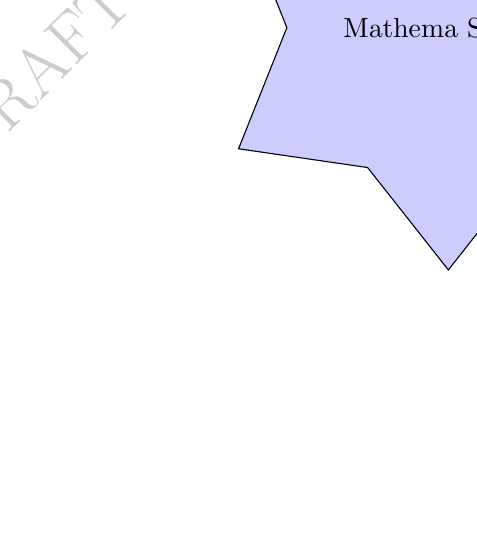
\begin{tikzpicture}
		\tikz \node [fill=blue!20,star,star points=6,draw] {Mathema Shukur };
	\end{tikzpicture}
	\\
	যাদের জন্যে প্রযোজ্যঃ  	\textcolor{magenta}{একাদশ ও দ্বাদশ শ্রেণীর শিক্ষার্থী} \\
	বিষয়ঃ \textcolor{magenta}{উচ্চতর গণিত ১ম পত্র} \\
	অধ্যায়ঃ \textcolor{magenta}{৩-সরলরেখা}\\ 
	Subtopicঃ  \textcolor{magenta}{ ত্রিভুজের অন্তঃ কেন্দ্র নির্ণয় করা }\\
	\\
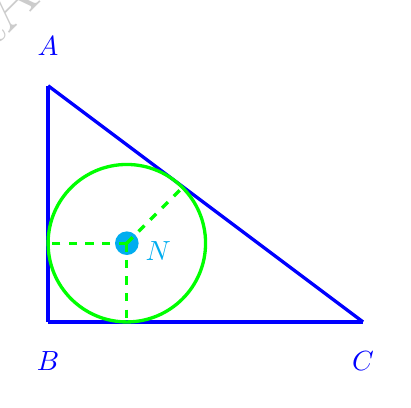
\begin{tikzpicture}[transform shape,scale=1]
	\fill[cyan] (1,1) circle (1.5 mm);
	\node at (1.4,0.9) {$\textcolor{cyan}{N}$};	
	\draw[very thick,blue] (0,0)--(0,3);
	\node at (0,-0.5) {$\textcolor{blue}{B}$};		
	\node at (0,3.5) {$\textcolor{blue}{A}$};	
	\draw[very thick,blue] (0,3)--(4,0);
	\node at (4,-0.5) {$\textcolor{blue}{C}$};		
	\draw[very thick,blue] (0,0)--(4,0);		
	\draw[very thick,green,dashed] (1,1)--(1.7,1.7);				
	\draw[very thick,green,dashed] (1,1)--(0,1);	
	\draw[very thick,green,dashed] (1,1)--(1,0);		
	\draw[very thick,green] (1,1) circle (1);			
\end{tikzpicture}
\\
ত্রিভুজের অন্তঃস্থ বৃত্তের কেন্দ্রকে অন্তঃ কেন্দ্র বলে। বৃত্তের ব্যাসার্ধের ধারণা থেকে বলা যায়  অন্তকেন্দ্র থেকে ত্রিভুজের তিনটি বাহুর লম্ব দূরত্ব সমান। ত্রিভুজের তিনটি বাহু বৃত্তের স্পর্শক হিসাবে বিদ্যমান। \\
	\\ 
		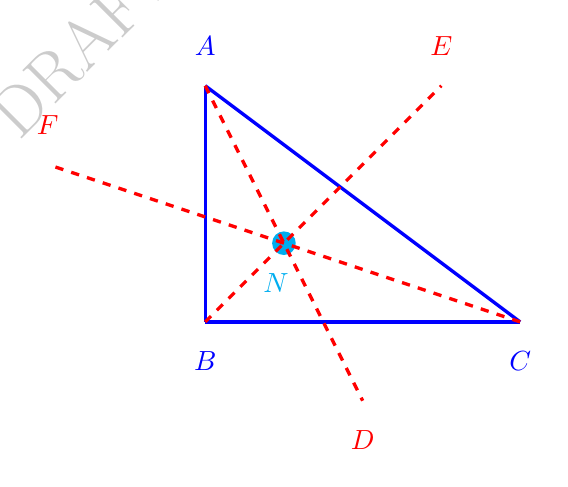
\begin{tikzpicture}[transform shape,scale=1]
		\fill[cyan] (1,1) circle (1.5 mm);
			\node at (0.9,0.5) {$\textcolor{cyan}{N}$};	
		\draw[very thick,blue] (0,0)--(0,3);
			\node at (0,-0.5) {$\textcolor{blue}{B}$};		
			\node at (0,3.5) {$\textcolor{blue}{A}$};	
		\draw[very thick,blue] (0,3)--(4,0);
			\node at (4,-0.5) {$\textcolor{blue}{C}$};		
		\draw[very thick,blue] (0,0)--(4,0);		
			\draw[very thick,red,dashed] (0,0)--(3,3);	
					\node at (3,3.5) {$\textcolor{red}{E}$};			
				\draw[very thick,red,dashed] (4,0)--(-2,2);	
				\node at (-2,2.5) {$\textcolor{red}{F}$};	
				\draw[very thick,red,dashed] (0,3)--(2,-1);	
				\node at (2,-1.5) {$\textcolor{red}{D}$};	
	\end{tikzpicture}
\\ 
ত্রিভুজের তিনটি কোণের  তিনটি সমদ্বিখন্ডক যে বিন্দুতে মিলিত হয় তাকে অন্তঃ কেন্দ্র বলে। \\
\\
\\
\\
	$A$ কোণের বিপরীত বাহুর দৈর্ঘ্য   $BC=a$ \\
	$B$ কোণের বিপরীত বাহুর দৈর্ঘ্য    $AC=b$ \\
	$C$ কোণের বিপরীত বাহুর দৈর্ঘ্য   $AB=c$\\
	\\ 
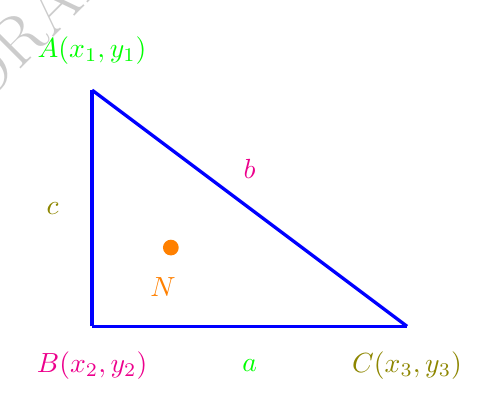
\begin{tikzpicture}[transform shape,scale=1]
	\fill[orange] (1,1) circle (1 mm);
	\node at (0.9,0.5) {$\textcolor{orange}{N}$};	
	\draw[very thick,blue] (0,0)--(0,3);
	\node at (0,-0.5) {$\textcolor{magenta}{B(x_2,y_2)}$};		
	\node at (0,3.5) {$\textcolor{green}{A(x_1,y_1)}$};	
	\draw[very thick,blue] (0,3)--(4,0);
	\node at (4,-0.5) {$\textcolor{olive}{C(x_3,y_3)}$};		
	\draw[very thick,blue] (0,0)--(4,0);		
	\node at (2,2) {$\textcolor{magenta}{b}$};			
	\node at (-0.5,1.5) {$\textcolor{olive}{c}$};	
	\node at (2,-0.5) {$\textcolor{green}{a}$};	
\end{tikzpicture}
\\ 
অন্তঃ কেন্দ্রের স্থানাঙ্ক \\ 
\[N\left(\frac{\textcolor{green}{a\,x_1}+\textcolor{magenta}{b\,x_2}+\textcolor{olive}{c\,x_3}}{\textcolor{green}{a}+\textcolor{magenta}{b}+\textcolor{olive}{c}},\frac{\textcolor{green}{a\,y_1}+\textcolor{magenta}{b\,y_2}+\textcolor{olive}{c\,y_3}}{\textcolor{green}{a}+\textcolor{magenta}{b}+\textcolor{olive}{c}}\right)\]
\\ 
\\ 
যে ত্রিভুজের বাহুগুলির সমীকরণ 	$2x-y-1=0$,  $x+2y-8=0$ এবং  $11x+2y+32=0$; তার অন্তঃকেন্দ্র নির্ণয় কর \\
\\  
	\begin{tikzpicture}[transform shape,scale=1]
		\draw [-latex,thick](-6,0) -- (6,0) node[right] {$x$} coordinate(x axis);
		\draw [-latex,thick](0,-6) -- (0,6) node[above] {$y$} coordinate(y axis);
		\fill[cyan] (-1,2) circle (1 mm);
		\node at (2,-1) {$\textcolor{green}{2x-y-1=0}$};		
		\node at (2,4) {$\textcolor{red}{x+2y-8=0}$};	
		\node at (-5,-1) {$\textcolor{blue}{11x+2y+32=0}$};	
			\node at (-4,6.3) {$\textcolor{blue}{B}$};		
		\node at (2.3,3) {$\textcolor{blue}{A}$};	
			\node at (-2,-5.4) {$\textcolor{blue}{C}$};	
		\draw[very thick,green] (2,3)--(-2,-5);	
		\draw[very thick,blue] (-2,-5)--(-4,6);	
		\draw[very thick,red] (2,3)--(-4,6);		
	\end{tikzpicture}
\vspace{2cm}
\begin{multicols}{3}
$A$ বিন্দুর স্থানাঙ্ক নির্ণয়  \\
\\
$AB : \,\, x+2y-8=0$ \\
\\
$AC: 2x-y-1=0$\\
\\ 
$AB$ ও $AC$ এর সমাধান $\textcolor{blue}{(x_1,y_1)=(2,3)}$\\
\\
\\
$B$ বিন্দুর স্থানাঙ্ক নির্ণয়  \\
\\
$AB : \,\, x+2y-8=0$ \\
\\
$BC:\,\,\,11x+2y+32=0$\\
\\
$AB$ ও $BC$ এর সমাধান $\textcolor{blue}{(x_2,y_2)=(-4,6)}$\\
\\
$C$ বিন্দুর স্থানাঙ্ক নির্ণয়  \\
\\
$AC: 2x-y-1=0$\\
\\ 
$BC:\,\,\,11x+2y+32=0$\\
\\
$AC$ ও $BC$ এর সমাধান $\textcolor{blue}{(x_3,y_3)=(-2,-5)}$\\
\end{multicols}
$A$ কোণের বিপরীত বাহুর দৈর্ঘ্য   $B(-4,6)C(-2,-5)=a=\sqrt{(-4+2)^2+(6+5)^2}=5\sqrt{5}$ \\
\\
$B$ কোণের বিপরীত বাহুর দৈর্ঘ্য    $A(2,3)C(-2,-5)=b=\sqrt{(2+2)^2+(3+5)^2}=4\sqrt{5}$ \\
\\
$C$ কোণের বিপরীত বাহুর দৈর্ঘ্য   $A(2,3)B(-4,6)=c=\sqrt{(2+4)^2+(3-6)^2}=3\sqrt{5}$\\
\\
 ত্রিভুজ $ABC$ এর অন্তঃ কেন্দ্রের স্থানাঙ্ক \\ 
\begin{align*}
	&\left(\frac{a\,\,x_1+b\,\,x_2+c\,\,x_3}{a+b+c},\frac{a\,\,y_1+b\,\,y_2+c\,\,y_3}{a+b+c},\right)\\
	\\
	&\left(\frac{5\sqrt{5}\,\,(2)+4\sqrt{5}\,\,(-4)+3\sqrt{5}\,\,(-2)}{5\sqrt{5}+4\sqrt{5}+3\sqrt{5}},\frac{5\sqrt{5}\,\,(3)+4\sqrt{5}\,\,(6)+3\sqrt{5}\,\,(-5)}{5\sqrt{5}+4\sqrt{5}+3\sqrt{5}}\right)\\
	\\
		&\left(\frac{10\sqrt{5}-16\sqrt{5}-6\sqrt{5}}{12\sqrt{5}},\frac{15\sqrt{5}+24\sqrt{5}-15\sqrt{5}}{12\sqrt{5}}\right)\\
		\\
			&\left(\frac{-12\sqrt{5}}{12\sqrt{5}},\frac{24\sqrt{5}}{12\sqrt{5}}\right)\\
		\\
		&(-1,2)
\end{align*}
	যশোর  বোর্ড-২০২১\\ 
যে ত্রিভুজের বাহুগুলির সমীকরণ 	$4x+3y-12=0$,  $3x-4y+16=0$ এবং  $4x-3y-12=0$; তার অন্তঃকেন্দ্র নির্ণয় কর \\
\\ 
$\left(3,\frac{25}{7}\right)$\\
\end{document}